\documentclass{article}
\usepackage{amsfonts}
\usepackage{amsmath}
\usepackage{graphicx}

\setlength{\parindent}{0pt}
\setlength{\parskip}{5pt}
\title{HW Week 4}
\author{Max Horowitz-Gelb}
\date{2/11/17}
\begin{document}
\maketitle
\section*{Q1}
Let $X$ be a THMC Markhov random variable.
Then let our transition matrix be described,
\[
p(i,j) = 
\begin{cases}
1 & j = i + 1 \\
0 & else
\end{cases}
\]
Clearly then for all $n \geq 1$, $Xn = X_{n-1} + 1$ with probability 1,
and for any state $i$, $\rho(i,i) = 0$. Therefore for any state $i$, $i$ is transient. 

\section*{Q2}
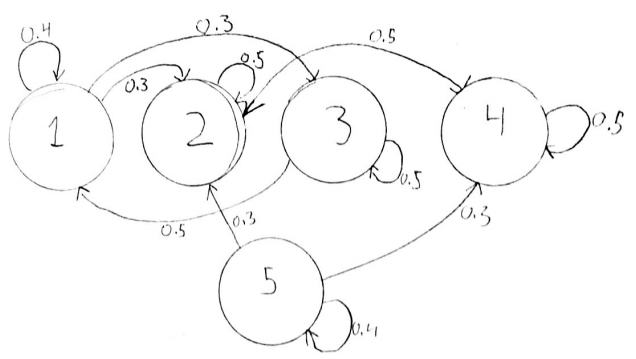
\includegraphics[scale=0.75]{transition.png}
State $1$ has a $0.3$ probability of transitioning to state $2$ and there is no path from state $2$ to state $1$. Therefore $\rho(1,1) \leq 0.7 < 1$ and state $1$ is transient.

State 3 has a 0.5 probability of transitioning into state 1, and state 1 is the only state besides state 3 that can transition into state 3. Therefore, since state 1 is transient, then state 3 is transient. This is because if state 3 were recurrent, then $\rho(3,3) = 1$, and since $p(3,1) > 0$, then this would imply $\rho(3,1) = 1$. But state 1 has a 0.3 probability of transitioning to state 2 and state 2 has no transition path to state 1 or 3. This would imply that $\rho(1,3) < 1$, which is a contradiction since $\rho(3,1) = 1$ and $\rho(1,3) < 1$ implies that $\rho(3,3) < 1$.                                                                                                                                                                                                                                                                                                                                                                                                                                                                                                                                                                                                                                                                                                                                                                                                                                                                                                                                                                                                                                                                                                                                                                                                                                                                                                                                                                                                                                                                                                                                                                                                                                                                                                                                                                                                                                                                                                                                                                                                                                                                                                                                                                                                                                                                                                                                                                                                                                                                                                                                                                                                                                                                                                                                                                                                                                                                                                                                                                                                                                                                                                                                                                                                                                                                                                                                                                                                                                                                                                                                                                                                                                                       

State 5 is transient since there is a 0.6 probability of transitioning from state 5 to state 2 or 4 and there is no transition path from 2 or 4 back to state 5.                                                                                                                                                                                                                                                                                                                                                                                                                                                                                                                                                                                                                                                                                                                                                                                                                                                                                                                                                                                                                                                                                                                                                                                                                                                                                                                                                                                                                                                                                                                                                                                                                                                                                                                                                                                                                                                                                                                                                                                                                                                                                        

\section*{Q3}
\subsection*{b}
States 1, 4, 5 and 6 are in an irreducible closed set. This is because for any pair in that set, there is a transition path between them. As well, there are no transitions out of that set into the remaining states 2 and 3. There is no irreducible closed set that contains either state 2 or 3, since there are transitions out of those states into states 1, 5 and 6, but there are no transition paths from 1, 5 and 6 back to state 2 or 3. Then since there are a finite set of states and 1, 4, 5 and 6 are in a irreducible closed set, then by theorem 1.7, they are all recurrent. And 2 and 3 do not exist in any irreducible closed set, so by the same theorem they must be transient.

\subsection*{d}
States 1 and 4 are in an irreducible closed set since they both have transitions to each-other and no outgoing transitions. For the same reasons, states 5 and 2 are in an irreducible closed set. No other states can be places in such a set and since there are a finite number of states, then by theorem 1.7, 1, 4, 5 and 2 are recurrent states, and 3 and 6 are transient.  


\end{document}


